% I seguenti commenti speciali impostano:
% 1. 
% 2. PDFLaTeX come motore di composizione;
% 3. tesi.tex come documento principale;
% 4. il controllo ortografico italiano per l'editor.

% !TEX encoding = UTF-8
% !TEX TS-program = pdflatex
% !TEX root = tesi.tex
% !TEX spellcheck = it-IT

\documentclass[10pt,                    % corpo del font principale
               a4paper,                 % carta A4
               twoside,                 % impagina per fronte-retro
               openright,               % inizio capitoli a destra
               english,                 
               italian,                 
               ]{book}    

%**************************************************************
% Importazione package
%************************************************************** 

%\usepackage{amsmath,amssymb,amsthm}    % matematica

\usepackage[T1]{fontenc}                % codifica dei font:
                                        % NOTA BENE! richiede una distribuzione *completa* di LaTeX

\usepackage[utf8]{inputenc}             % codifica di input; anche [latin1] va bene
                                        % NOTA BENE! va accordata con le preferenze dell'editor

\usepackage[english, italian]{babel}    % per scrivere in italiano e in inglese;
                                        % l'ultima lingua (l'italiano) risulta predefinita

\usepackage{bookmark}                   % segnalibri

\usepackage{caption}                    % didascalie

\usepackage{chngpage,calc}              % centra il frontespizio

\usepackage{csquotes}                   % gestisce automaticamente i caratteri (")

\usepackage{emptypage}                  % pagine vuote senza testatina e piede di pagina

\usepackage{epigraph}			% per epigrafi

\usepackage{eurosym}                    % simbolo dell'euro

%\usepackage{indentfirst}               % rientra il primo paragrafo di ogni sezione

\usepackage{graphicx}                   % immagini

\usepackage{hyperref}                   % collegamenti ipertestuali

\usepackage[binding=5mm]{layaureo}      % margini ottimizzati per l'A4; rilegatura di 5 mm

\usepackage{listings}                   % codici

\usepackage{microtype}                  % microtipografia

\usepackage{mparhack,fixltx2e,relsize}  % finezze tipografiche

\usepackage{nameref}                    % visualizza nome dei riferimenti                                      

\usepackage[font=small]{quoting}        % citazioni

\usepackage{subfig}                     % sottofigure, sottotabelle

\usepackage[italian]{varioref}          % riferimenti completi della pagina

\usepackage[dvipsnames]{xcolor}         % colori

\usepackage{booktabs}                   % tabelle                                       
\usepackage{tabularx}                   % tabelle di larghezza prefissata                                    
\usepackage{longtable}                  % tabelle su più pagine                                        
\usepackage{ltxtable}                   % tabelle su più pagine e adattabili in larghezza

\usepackage[toc, acronym]{glossaries}   % glossario
                                        % per includerlo nel documento bisogna:
                                        % 1. compilare una prima volta tesi.tex;
                                        % 2. eseguire: makeindex -s tesi.ist -t tesi.glg -o tesi.gls tesi.glo
                                        % 3. eseguire: makeindex -s tesi.ist -t tesi.alg -o tesi.acr tesi.acn
                                        % 4. compilare due volte tesi.tex.

\usepackage[backend=biber,style=verbose-ibid,hyperref,backref]{biblatex}
                                        % eccellente pacchetto per la bibliografia; 
                                        % produce uno stile di citazione autore-anno; 
                                        % lo stile "numeric-comp" produce riferimenti numerici
                                        % per includerlo nel documento bisogna:
                                        % 1. compilare una prima volta tesi.tex;
                                        % 2. eseguire: biber tesi
                                        % 3. compilare ancora tesi.tex.

%**************************************************************
% file contenente le impostazioni della tesi
%**************************************************************

%**************************************************************
% Frontespizio
%**************************************************************

% Autore
\newcommand{\myName}{Alessandro Discalzi}                                    
\newcommand{\myTitle}{Advertising management system: Creazione e gestione di contenuti pubblicitari}

% Tipo di tesi                   
\newcommand{\myDegree}{Tesi di laurea}

% Università             
\newcommand{\myUni}{Università degli Studi di Padova}

% Facoltà       
\newcommand{\myFaculty}{Corso di Laurea in Informatica}

% Dipartimento
\newcommand{\myDepartment}{Dipartimento di Matematica "Tullio Levi-Civita"}

% Titolo del relatore
\newcommand{\profTitle}{Prof. }

% Relatore
\newcommand{\myProf}{Claudio Enrico Palazzi}

% Luogo
\newcommand{\myLocation}{Padova}

% Anno accademico
\newcommand{\myAA}{2019-2020}

% Data discussione
\newcommand{\myTime}{Settembre 2020}


%**************************************************************
% Impostazioni di impaginazione
% see: http://wwwcdf.pd.infn.it/AppuntiLinux/a2547.htm
%**************************************************************

\setlength{\parindent}{14pt}   % larghezza rientro della prima riga
\setlength{\parskip}{0pt}   % distanza tra i paragrafi


%**************************************************************
% Impostazioni di biblatex
%**************************************************************
\bibliography{bibliografia} % database di biblatex 

\defbibheading{bibliography} {
    \cleardoublepage
    \phantomsection 
    \addcontentsline{toc}{chapter}{\bibname}
    \chapter*{\bibname\markboth{\bibname}{\bibname}}
}

\setlength\bibitemsep{1.5\itemsep} % spazio tra entry

\DeclareBibliographyCategory{opere}
\DeclareBibliographyCategory{web}

\addtocategory{opere}{womak:lean-thinking}
\addtocategory{web}{site:agile-manifesto}

\defbibheading{opere}{\section*{Riferimenti bibliografici}}
\defbibheading{web}{\section*{Siti Web consultati}}


%**************************************************************
% Impostazioni di caption
%**************************************************************
\captionsetup{
    tableposition=top,
    figureposition=bottom,
    font=small,
    format=hang,
    labelfont=bf
}

%**************************************************************
% Impostazioni di glossaries
%**************************************************************

%**************************************************************
% Acronimi
%**************************************************************
\renewcommand{\acronymname}{Acronimi e abbreviazioni}

\newacronym[description={\glslink{apig}{Application Program Interface}}]
    {api}{API}{Application Program Interface}

\newacronym[description={\glslink{umlg}{Unified Modeling Language}}]
    {uml}{UML}{Unified Modeling Language}

%**************************************************************
% Glossario
%**************************************************************
%\renewcommand{\glossaryname}{Glossario}

\newglossaryentry{apig}
{
    name=\glslink{api}{API},
    text=Application Program Interface,
    sort=api,
    description={in informatica con il termine \emph{Application Programming Interface API} (ing. interfaccia di programmazione di un'applicazione) si indica ogni insieme di procedure disponibili al programmatore, di solito raggruppate a formare un set di strumenti specifici per l'espletamento di un determinato compito all'interno di un certo programma. La finalità è ottenere un'astrazione, di solito tra l'hardware e il programmatore o tra software a basso e quello ad alto livello semplificando così il lavoro di programmazione}
}

\newglossaryentry{umlg}
{
    name=\glslink{uml}{UML},
    text=UML,
    sort=uml,
    description={in ingegneria del software \emph{UML, Unified Modeling Language} (ing. linguaggio di modellazione unificato) è un linguaggio di modellazione e specifica basato sul paradigma object-oriented. L'\emph{UML} svolge un'importantissima funzione di ``lingua franca'' nella comunità della progettazione e programmazione a oggetti. Gran parte della letteratura di settore usa tale linguaggio per descrivere soluzioni analitiche e progettuali in modo sintetico e comprensibile a un vasto pubblico}
}

\newglossaryentry{systemIntegratorg}
{
    name=\glslink{System Integrator}{system integrator},
    text=System Integrator,
    sort=system Integrator,
    description=asd
}

\newglossaryentry{contenutog}
{
    name=\glslink{Contenuto informativo}{contenuto informativo},
    text=contenuti informativi,
    sort=contenuto informativo,
    description=asd
}

\newglossaryentry{cloudnativog}
{
    name=\glslink{Cloud nativo}{cloud nativo},
    text=Cloud nativo,
    sort=cloud nativo,
    description=asd
}

\newglossaryentry{appserverg}
{
    name=\glslink{Application server}{application server},
    text=Application server,
    sort=application server,
    description=asd
}

\newglossaryentry{microservizig}
{
    name=\glslink{Microservizi}{microservizi},
    text=Microservizi,
    sort=microservizi,
    description=asd
}

\newglossaryentry{iocg}
{
    name=\glslink{Inversione di controllo}{inversione di controllo},
    text=inversione di controllo,
    sort=inversione di controllo,
    description=asd
}

\newglossaryentry{dbmsg}
{
    name=\glslink{DBMS}{dbms},
    text=DBMS,
    sort=dbms,
    description=asd
}

\newglossaryentry{ui}
{
    name=\glslink{UI}{ui},
    text=UI,
    sort=ui,
    description=asd
}

\newglossaryentry{ux}
{
    name=\glslink{UX}{ux},
    text=UX,
    sort=ux,
    description=asd
}

\newglossaryentry{ci}
{
    name=\glslink{CI}{ci},
    text=CI,
    sort=ci,
    description=asd
}

\newglossaryentry{ssog}
{
    name=\glslink{SSO}{sso},
    text=SSO,
    sort=sso,
    description=asd
}

\newglossaryentry{mockg}
{
    name=\glslink{Mock}{mock},
    text=Mock,
    sort=mock,
    description=asd
} % database di termini
\makeglossaries


%**************************************************************
% Impostazioni di graphicx
%**************************************************************
\graphicspath{{immagini/}} % cartella dove sono riposte le immagini


%**************************************************************
% Impostazioni di hyperref
%**************************************************************
\hypersetup{
    %hyperfootnotes=false,
    %pdfpagelabels,
    %draft,	% = elimina tutti i link (utile per stampe in bianco e nero)
    colorlinks=true,
    linktocpage=true,
    pdfstartpage=1,
    pdfstartview=FitV,
    % decommenta la riga seguente per avere link in nero (per esempio per la stampa in bianco e nero)
    %colorlinks=false, linktocpage=false, pdfborder={0 0 0}, pdfstartpage=1, pdfstartview=FitV,
    breaklinks=true,
    pdfpagemode=UseNone,
    pageanchor=true,
    pdfpagemode=UseOutlines,
    plainpages=false,
    bookmarksnumbered,
    bookmarksopen=true,
    bookmarksopenlevel=1,
    hypertexnames=true,
    pdfhighlight=/O,
    %nesting=true,
    %frenchlinks,
    urlcolor=webbrown,
    linkcolor=RoyalBlue,
    citecolor=webgreen,
    %pagecolor=RoyalBlue,
    %urlcolor=Black, linkcolor=Black, citecolor=Black, %pagecolor=Black,
    pdftitle={\myTitle},
    pdfauthor={\textcopyright\ \myName, \myUni, \myFaculty},
    pdfsubject={},
    pdfkeywords={},
    pdfcreator={pdfLaTeX},
    pdfproducer={LaTeX}
}

%**************************************************************
% Impostazioni di itemize
%**************************************************************
\renewcommand{\labelitemi}{$\bullet$}

%**************************************************************
% Impostazioni di listings
%**************************************************************
\lstset{
    language=[LaTeX]Tex,%C++,
    keywordstyle=\color{RoyalBlue}, %\bfseries,
    basicstyle=\small\ttfamily,
    %identifierstyle=\color{NavyBlue},
    commentstyle=\color{Green}\ttfamily,
    stringstyle=\rmfamily,
    numbers=none, %left,%
    numberstyle=\scriptsize, %\tiny
    stepnumber=5,
    numbersep=8pt,
    showstringspaces=false,
    breaklines=true,
    frameround=ftff,
    frame=single
} 


%**************************************************************
% Impostazioni di xcolor
%**************************************************************
\definecolor{webgreen}{rgb}{0,.5,0}
\definecolor{webbrown}{rgb}{.6,0,0}


%**************************************************************
% Altro
%**************************************************************

\newcommand{\omissis}{[\dots\negthinspace]} % produce [...]

% eccezioni all'algoritmo di sillabazione
%*\hyphenation{}

\newcommand{\sectionname}{sezione}
\addto\captionsitalian{\renewcommand{\figurename}{Figura}
                       \renewcommand{\tablename}{Tabella}}

\newcommand{\glsfirstoccur}{\ap{{[g]}}}

\newcommand{\intro}[1]{\emph{\textsf{#1}}}

%**************************************************************
% Environment per ``rischi''
%**************************************************************
\newcounter{riskcounter}                % define a counter
\setcounter{riskcounter}{0}             % set the counter to some initial value

%%%% Parameters
% #1: Title
\newenvironment{risk}[1]{
    \refstepcounter{riskcounter}        % increment counter
    \par \noindent                      % start new paragraph
    \textbf{\arabic{riskcounter}. #1}   % display the title before the 
                                        % content of the environment is displayed 
}{
    \par\medskip
}

\newcommand{\riskname}{Rischio}

\newcommand{\riskdescription}[1]{\textbf{\\Descrizione:} #1.}

\newcommand{\risksolution}[1]{\textbf{\\Soluzione:} #1.}

%**************************************************************
% Environment per ``use case''
%**************************************************************
\newcounter{usecasecounter}             % define a counter
\setcounter{usecasecounter}{0}          % set the counter to some initial value

%%%% Parameters
% #1: ID
% #2: Nome
\newenvironment{usecase}[2]{
    \renewcommand{\theusecasecounter}{\usecasename #1}  % this is where the display of 
                                                        % the counter is overwritten/modified
    \refstepcounter{usecasecounter}             % increment counter
    \vspace{10pt}
    \par \noindent                              % start new paragraph
    {\large \textbf{\usecasename #1: #2}}       % display the title before the 
                                                % content of the environment is displayed 
    \medskip
}{
    \medskip
}

\newcommand{\usecasename}{UC}

\newcommand{\usecaseactors}[1]{\textbf{\\Attori Principali:} #1. \vspace{4pt}}
\newcommand{\usecasepre}[1]{\textbf{\\Precondizioni:} #1. \vspace{4pt}}
\newcommand{\usecasedesc}[1]{\textbf{\\Descrizione:} #1. \vspace{4pt}}
\newcommand{\usecasepost}[1]{\textbf{\\Postcondizioni:} #1. \vspace{4pt}}
\newcommand{\usecasealt}[1]{\textbf{\\Scenario Alternativo:} #1. \vspace{4pt}}

%**************************************************************
% Environment per ``namespace description''
%**************************************************************

\newenvironment{namespacedesc}{
    \vspace{10pt}
    \par \noindent                              % start new paragraph
    \begin{description} 
}{
    \end{description}
    \medskip
}

\newcommand{\classdesc}[2]{\item[\textbf{#1:}] #2}
                     % file con le impostazioni personali

\begin{document}
%**************************************************************
% Materiale iniziale
%**************************************************************
\frontmatter
% !TEX encoding = UTF-8
% !TEX TS-program = pdflatex
% !TEX root = ../tesi.tex

%**************************************************************
% Frontespizio 
%**************************************************************
\begin{titlepage}

\begin{center}

\begin{LARGE}
\textbf{\myUni}\\
\end{LARGE}

\vspace{10pt}

\begin{Large}
\textsc{\myDepartment}\\
\end{Large}

\vspace{10pt}

\begin{large}
\textsc{\myFaculty}\\
\end{large}

\vspace{29pt}
\begin{figure}[htbp]
\begin{center}

\includegraphics[height=6cm]{logo-unipd}
\end{center}
\end{figure}
\vspace{8pt} 

\begin{LARGE}
\begin{center}
\textbf{
    \begin{center}
        Advertising management system:
    \end{center} 
    Creazione e gestione di contenuti pubblicitari}\\
\end{center}
\end{LARGE}

\vspace{8pt} 

\begin{large}
\textsl{\myDegree}\\
\end{large}

\vspace{40pt} 

\begin{large}
\begin{flushleft}
\textit{Relatore}\\ 
\vspace{5pt} 
\profTitle \myProf
\end{flushleft}

\vspace{0pt} 

\begin{flushright}
\textit{Laureando}\\ 
\vspace{5pt} 
\myName
\end{flushright}
\end{large}

\vspace{40pt}

\line(1, 0){338} \\
\begin{normalsize}
\textsc{Anno Accademico \myAA}
\end{normalsize}

\end{center}
\end{titlepage} 
% !TEX encoding = UTF-8
% !TEX TS-program = pdflatex
% !TEX root = ../tesi.tex

%**************************************************************
% Colophon
%**************************************************************
\clearpage
\phantomsection
\thispagestyle{empty}

\hfill

\vfill

\noindent\myName: \textit{\myTitle,}
\myDegree,
\textcopyright\ \myTime.
%% !TEX encoding = UTF-8
% !TEX TS-program = pdflatex
% !TEX root = ../tesi.tex

%**************************************************************
% Dedica
%**************************************************************
\cleardoublepage
\phantomsection
\thispagestyle{empty}
\pdfbookmark{Dedica}{Dedica}

\vspace*{3cm}

\begin{center}
Lorem ipsum dolor sit amet, consectetuer adipiscing elit. \\ \medskip
--- Oscar Wilde    
\end{center}

\medskip

\begin{center}
Dedicato a ...
\end{center}

% !TEX encoding = UTF-8
% !TEX TS-program = pdflatex
% !TEX root = ../tesi.tex

%**************************************************************
% Sommario
%**************************************************************
\cleardoublepage
\phantomsection
\pdfbookmark{Sommario}{Sommario}
\begingroup
\let\clearpage\relax
\let\cleardoublepage\relax
\let\cleardoublepage\relax

\chapter*{Sommario}

Il presente documento descrive il lavoro svolto durante il periodo di stage dal laureando \myName presso l'azienda SCAI ITEC.
Lo stage è stato svolto al termine del percorso di studi della laurea triennale in informatica e la sua durata è stata di 312 ore.
L'obbiettivo dello stage è stato di implementare un applicativo per la creazione e per la gestione di contenuti pubblicitari.
Il presente documento vuole illustrare il contesto aziendale dove si è svolto lo stage, le attività svolte e una valutazione sul lavoro effettuato e su quanto appreso.

%\vfill
%
%\selectlanguage{english}
%\pdfbookmark{Abstract}{Abstract}
%\chapter*{Abstract}
%
%\selectlanguage{italian}

\endgroup			

\vfill


% !TEX encoding = UTF-8
% !TEX TS-program = pdflatex
% !TEX root = ../tesi.tex

%**************************************************************
% Ringraziamenti
%**************************************************************
\cleardoublepage
\phantomsection
\pdfbookmark{Ringraziamenti}{ringraziamenti}

\begin{flushright}{
	\slshape    
	``Nessuno ha mai ottenuto nulla con le lacrime.''} \\ 
	\medskip
    --- Brucaliffo
\end{flushright}


\bigskip

\begingroup
\let\clearpage\relax
\let\cleardoublepage\relax
\let\cleardoublepage\relax

\chapter*{Ringraziamenti}

\noindent \textit{Innanzitutto, vorrei esprimere la mia gratitudine al Prof. Claudio Enrico Palazzi, relatore della mia tesi, per l'aiuto e il sostegno che mi ha fornito durante la stesura del lavoro.}\\

\noindent \textit{Desidero ringraziare con affetto la mia famiglia, e in particolare i miei genitori per il sostegno e per il grande aiuto che mi hanno dato durante gli anni di studio.}\\

\noindent \textit{Desidero inoltre ringraziare il mio tutor aziendale, Dott. Bledar Gogaj, e il suo collega, Dott. Marco Lionello per l'enorme aiuto che mi hanno dato durante il periodo di stage.}\\

\noindent \textit{Un ringraziamento infine, ai miei amici per tutti i bei momenti passati insieme e per avermi sopportato tutti questi anni.}\\
\bigskip

\noindent\textit{\myLocation, \myTime}
\hfill \myName

\endgroup


% !TEX encoding = UTF-8
% !TEX TS-program = pdflatex
% !TEX root = ../tesi.tex

%**************************************************************
% Indici
%**************************************************************
\cleardoublepage
\pdfbookmark{\contentsname}{tableofcontents}
\setcounter{tocdepth}{2}
\tableofcontents
%\markboth{\contentsname}{\contentsname} 
\clearpage

\begingroup 
    \let\clearpage\relax
    \let\cleardoublepage\relax
    \let\cleardoublepage\relax
    %*******************************************************
    % Elenco delle figure
    %*******************************************************    
    \phantomsection
    \pdfbookmark{\listfigurename}{lof}
    \listoffigures

    \vspace*{8ex}

    %*******************************************************
    % Elenco delle tabelle
    %*******************************************************
    %\phantomsection
    %\pdfbookmark{\listtablename}{lot}
    %\listoftables
        
    \vspace*{8ex}
\endgroup

\cleardoublepage

\cleardoublepage

%**************************************************************
% Materiale principale
%**************************************************************
\mainmatter
% !TEX encoding = UTF-8
% !TEX TS-program = pdflatex
% !TEX root = ../tesi.tex

%**************************************************************
\chapter{Introduzione}
\label{cap:introduzione}
%**************************************************************

% Introduzione al contesto applicativo.\\

% \noindent Esempio di utilizzo di un termine nel glossario \\
% \gls{api}. \\

% \noindent Esempio di citazione in linea \\
% \cite{site:agile-manifesto}. \\

% \noindent Esempio di citazione nel pie' di pagina \\
%citazione\footcite{womak:lean-thinking} \\

%**************************************************************
\section{L'azienda}

\href{https://scaiitec.it/}{SCAI ITEC\footcite{SCAI ITEC abbrev: ITEC} } è un'azienda italiana appartenente al \href{https://www.grupposcai.it/}{gruppo SCAI}. ITEC si occupa di consulenza, System Integration ed Application management in ambito ICT. L'azienda opera principalmente in settore bancario, assicurativo, industriale e di pubblica amministrazione e servizi. \\Gli elementi chiave del successo e della crescita di SCAI ITEC sono:
\begin{itemize}
    \item vasta e profonda conoscenza delle tecnologie;
    \item grande attenzione per la soddisfazione del cliente;
    \item molta esperienza, maturata nel corso del tempo.
\end{itemize} 
ITEC è oggi una delle maggiori realtà nel nord-est del paese in ambito ICT e si propone come partner per qualsiasi tipo di applicazione, progetto e servizio modellato sulle specifiche necessità del cliente. 
\\Grazie alla consolidata esperienza nel ruolo di \gls{systemIntegratorg}\glsfirstoccur{} ed alle soluzioni leader di mercato proposte, ITEC è in grado di garantire ai propri clienti risposte rapide, concrete e qualificate in base alle specifiche esigenze di tipo gestionale e applicativo.
\\Ultimo, ma non meno importante, dei motivi per cui l'azienda è all'avanguardia rispetto le nuove tecnologie è il grande investimento di ITEC in ricerca, sviluppo e formazione del personale.

\begin{figure}[h]
    \begin{center}
    
\includegraphics[width=0.5\textwidth]{logo-itec}
    \caption{Logo SCAI ITEC}
    \label{fig:figure1}
    \end{center}
\end{figure}


%**************************************************************
\section{Scopo dello stage}
\label{sez:scopo}
L'obiettivo principale dello stage è stato quello di inserire lo studente all'interno di una nuova progettualità, con un particolare focus sulle tematiche legate alle tecnologie multimediali e alla loro distribuzione. Lo studente, affiancato da un IT Architect, ha avuto la possibilità di partecipare al disegno, alla progettazione e realizzazione di una nuova progettualità. L'obbiettivo è stato apprendere le tecnologie e le best practice utilizzate in azienda nel ciclo di vita di un applicativo.
La progettualità vista è volta a creare un software per la gestione di \gls{contenutog}\glsfirstoccur{}, per la loro creazione, modifica e distribuzione nei vari canali di vendita.
Grazie a questa nuova applicazione si potrà:
\begin{itemize}
    \item creare, modificare eliminare e clonare dei contenuti informativi;
    \item raggruppare i contenuti informativi su segmenti di mercato e distribuirli;
    \item pianificare l’esecuzione e l’aggiornamento dei contenuti informativi sui vari canali di distribuzione;
    \item seguire un processo di Authoring (paradigma Editore, Redattore, Supervisore) nella fase di creazione e distribuzione.
\end{itemize} 
In quanto l'intero progetto è di dimensione non indifferente l'obbiettivo dello stage è stato di sviluppare le funzionalità relative al ruolo di Editore, più nello specifico:
\begin{itemize}
    \item creazione di un contenuto;
    \item modifica di un contenuto;
    \item eliminazione di un contenuto;
    \item preparazione di un contenuto per la distribuzione;
    \item auditing delle azioni effettuate dagli utenti;
    \item documentazione delle funzionalità implementate.
\end{itemize}

%**************************************************************
\section{Tecnologie utilizzate}

\subsection{JHipster}
\label{jhi}
\href{https://www.jhipster.tech/}{JHipster} è una piattaforma di sviluppo, con uno stack tecnologico ben definito, utilizzata per generare, sviluppare e rilasciare, applicazioni e web services all'avanguardia. Supporta molteplici tecnologie per il frontend, tra le quali Angular, React e Vue. Fornisce inoltre supporto per le applicazioni per dispositivi mobili utilizzando Ionic e React Native. Per quanto riguarda il backend, JHipster supporta spring Boot (con l'ausilio di Java o Kotlin), Micronaut, Quarkus, NodeJS e .NET. Per il rilascio sono adottati i principi di \gls{cloudnativog}\glsfirstoccur{}. Il rilascio è inoltre supportato su AWS, Azure, Cloud Foundry, Google Cloud Platform, Heroku ed OpenShift.
\\L'obbiettivo di JHipster è generare applicazioni web o microservizi all'avanguardia, unendo:
\begin{itemize}
    \item uno stack lato server robusto, ad alte prestazioni e coperto da test;
    \item un interfaccia utente accattivante, moderna e mobile-first usando Angular, React o Vue e Bootstrap per il CSS;
    \item un workflow ben definito per fare la build dell'applicazione con Maven o Gradle;
    \item un architettura a microservizi resiliente,  utilizzando i principi di \gls{cloudnativog};
    \item infrastruttura definita come codice, in modod da rendere la distribuzione su cloud veloce.
\end{itemize}
Nel corso dello stage JHipster è stato utilizzato per generare l'applicazione di base, utilizzata come punto di partenza per lo sviluppo.
\begin{figure}[h]
    \begin{center}
    
\includegraphics[width=0.18\textwidth]{logo-jhipster}
    \caption{Logo JHipster}
    \label{fig:figure2}
    \end{center}
\end{figure}

\subsection{Java Enterprise}
\href{https://www.oracle.com/it/java/technologies/java-ee-glance.html}{Java Enterprise}, conosciuto anche come Java EE è un insieme di specifiche che mirano ad estendere Java 8, aggiungendo funzionalità enterprise come elaborazione distribuita e servizi web. Le applicazioni Java EE possono essere eseguite sia come \gls{microservizig}\glsfirstoccur{} che su \gls{appserverg}\glsfirstoccur{}. In entrambi i casi vengono gestite: transazionalità, scalabilità, sicurezza e concorrenza.
Nel corso dello stage Java EE è stato utilizzato per la programmazione lato backend.
\begin{figure}[h]
    \begin{center}
    
\includegraphics[width=0.28\textwidth]{logo-javaee}
    \caption{Logo Java EE}
    \label{fig:figure3}
    \end{center}
\end{figure}

\subsection{Spring}
\href{https://spring.io/}{Spring} è un framework applicativo open source e un container per l'\gls{iocg}\glsfirstoccur{} utilizzato dalla piattaforma Java. Le funzionalità di base possono essere usate da una qualsiasi applicazione Java, mentre quelle più avanzate sono disponibili solamente per Java Enterprise.
Il framework Spring ha a se associati vari moduli, nel corso del progetto sono stati utilizzati principalmente:
\begin{itemize}
    \item Spring Boot: utilizzato per creare applicazioni basate su spring eseguibili senza la necessità di configurare un web server;
    \item Spring Data: il cui obbiettivo è di facilitare la gestione e l'interazione di applicazioni Java con un database.
\end{itemize}
\begin{figure}[h]
    \begin{center}
    
\includegraphics[width=0.35\textwidth]{logo-spring}
    \caption{Logo Spring}
    \label{fig:figure4}
    \end{center}
\end{figure}

\subsection{Hibernate}
\href{https://hibernate.org/}{Hibernate} è un framework per lo sviluppo di applicazioni in Java, utilizzato per gestire e mantenere su un database relazionale un insieme di oggetti Java.
\\Le sue funzionalità principali sono:
\begin{itemize}
    \item mappare oggetti Java come tabelle su database;
    \item convertire i campi dati Java a quelli del \gls{dbmsg}\glsfirstoccur{}{} utilizzato;
    \item generare chiamate SQL e convertire la risposta ottenuta in un oggetto Java.
\end{itemize}
Tali funzionalità sono state largamente utilizzate nel corso dello stage.
\begin{figure}[h]
    \begin{center}
    
\includegraphics[width=0.35\textwidth]{logo-hibernate}
    \caption{Logo Hibernate}
    \label{fig:figure5}
    \end{center}
\end{figure}

\subsection{REST\footcite{REST: acronimo di Representational State Transfer}}
\href{https://restfulapi.net/}{REST} è un modello architetturale per i sistemi distribuiti. I sistemi rest si basano su HTTP e prevedono una struttura degli URL ben definita, che identifichi univocamente le risorse secondo la convenzione del modello stesso\footcite{Resource Naming: https://restfulapi.net/resource-naming/}. 
In REST per il trasferimento di dati vengono utilizzati i metodi HTTP, più nello specifico:
\begin{itemize}
    \item GET: per il recupero di informazioni;
    \item POST, PUT, PATCH: per l'inserimento di informazioni;
    \item DELETE: per l'eliminazione di informazioni.
\end{itemize}
I principi guida di REST sono:
\begin{itemize}
    \item client-server: separazione dei problemi della UI da quelli di storage dei dati;
    \item statelessness: ogni richiesta deve avere tutte le informazioni necessarie per il suo processamento;
    \item cacheable: i client possono memorizzare in cache le risposte, queste devono essere definite esplicitamente o implicitamente cacheable, in modo da evitare il riutilizzo di dati errati;
    \item uniform interface: utilizzo di un'interfaccia di comunicazione omogenea tra client e server in modo da disaccoppiare e semplificare l'architettura per poterla modificare a blocchi;
    \item layered system:la struttura del sistema può essere composta da strati gerarchici. In questo caso ogni componente non può "vedere" oltre lo strato con cui sta interagendo;
    \item code on demand(opzionale): il codice lato client può essere esteso scaricando ed eseguendo applet o script.
\end{itemize}
Nella definizione di API se queste rispettano tutti i vincoli imposti dall'architettura REST allora possono essere definite RESTful.
\begin{figure}[h]
    \begin{center}
    
\includegraphics[width=0.2\textwidth]{logo-rest}
    \caption{Logo REST}
    \label{fig:figure6}
    \end{center}
\end{figure}

\subsection{Oracle}
\label{oracle}
\href{https://www.oracle.com/it/database/}{Oracle database} è un \gls{dbmsg} di tipo relazionale prodotto da \href{https://www.oracle.com/}{Oracle corporation}. 
\\I database oracle sono noti per offrire performance, scalabilità, affidabilità e sicurezza oltre a poter essere utilizzati sia on premise che nel cloud.
\begin{figure}[h]
    \begin{center}
    
\includegraphics[width=0.22\textwidth]{logo-oracle}
    \caption{Logo Oracle}
    \label{fig:figure7}
    \end{center}
\end{figure}

\subsection{Liquibase}
\href{https://www.liquibase.org/}{Liquibase} è una libreria open source indipendente dal \gls{dbmsg} utilizzato. Durante il periodo di stage è stata utilizzata per tracciare, gestire e applicare le modifiche allo schema del database.
\begin{figure}[h]
    \begin{center}
    
\includegraphics[width=0.23\textwidth]{logo-liquibase}
    \caption{Logo Liquibase}
    \label{fig:figure8}
    \end{center}
\end{figure}
\subsection{Angular}
\href{https://angular.io/}{Angular} è un framework open source per la progettazione e lo sviluppo di applicazioni web.
Le applicazioni angular vengono eseguite interamente a lato client ma grazie alla moltitudine di moduli presenti è possibile integrare un sistema di backend più complesso eseguito lato server.
Nel corso dello stage, il frontend, è stato scritto interamente in Angular.
\begin{figure}[h]
    \begin{center}
    
\includegraphics[width=0.23\textwidth]{logo-angular}
    \caption{Logo Angular}
    \label{fig:figure9}
    \end{center}
\end{figure}

%**************************************************************
\newpage
\section{Strumenti di sviluppo}

\subsection{Eclipse}
\label{eclipse}
L'IDE utilizzato per lo sviluppo, previo consiglio del tutor aziendale, è stato \href{https://www.eclipse.org/}{Eclipse}.
Eclipse è un ambiente di sviluppo integrato multipiattaforma e rientra nella categoria di software libero, distribuito secondo i termini della \href{https://www.eclipse.org/legal/epl-2.0/}{Eclipse Public License}.
\begin{figure}[h]
    \begin{center}
    
\includegraphics[width=0.35\textwidth]{logo-eclipse}
    \caption{Logo Eclipse}
    \label{fig:figure10}
    \end{center}
\end{figure}

\subsection{Maven}
\label{maven}
\href{https://maven.apache.org/}{Maven} è uno strumento di gestione di progetti software, è basato su un Project Object Model (POM) e può gestire la build, il reporting e la documentazione di un progetto. Nel corso dello stage Maven è stato utilizzato principalmente per automatizzare la build del progetto, sia in sviluppo che in produzione.
\begin{figure}[h]
    \begin{center}
    
\includegraphics[width=0.3\textwidth]{logo-maven}
    \caption{Logo Maven}
    \label{fig:figure11}
    \end{center}
\end{figure}

\subsection{Git}
\label{git}
\href{https://git-scm.com/}{Git} è un sistema di controllo di versione distribuito, gratuito ed open source, progettato per gestire progetti di qualsiasi tipo. Nel corso dello stage l'utilizzo di Git è stato affiancato a quello di GitLab, una piattaforma web per la gestione di repository Git.
\begin{figure}[h]
    \begin{center}
    
\includegraphics[width=0.2\textwidth]{logo-git}
    \caption{Logo Git}
    \label{fig:figure12}
    \end{center}
\end{figure}
\subsection{SQL Developer}
\href{https://www.oracle.com/database/technologies/appdev/sqldeveloper-landing.html}{SQL Developer} è un ambiente di sviluppo integrato per lavorare con SQL nei database Oracle. Nel corso dello stage è stato utilizzato per gestire e testare il database Oracle usato in produzione.
\begin{figure}[h]
    \begin{center}
    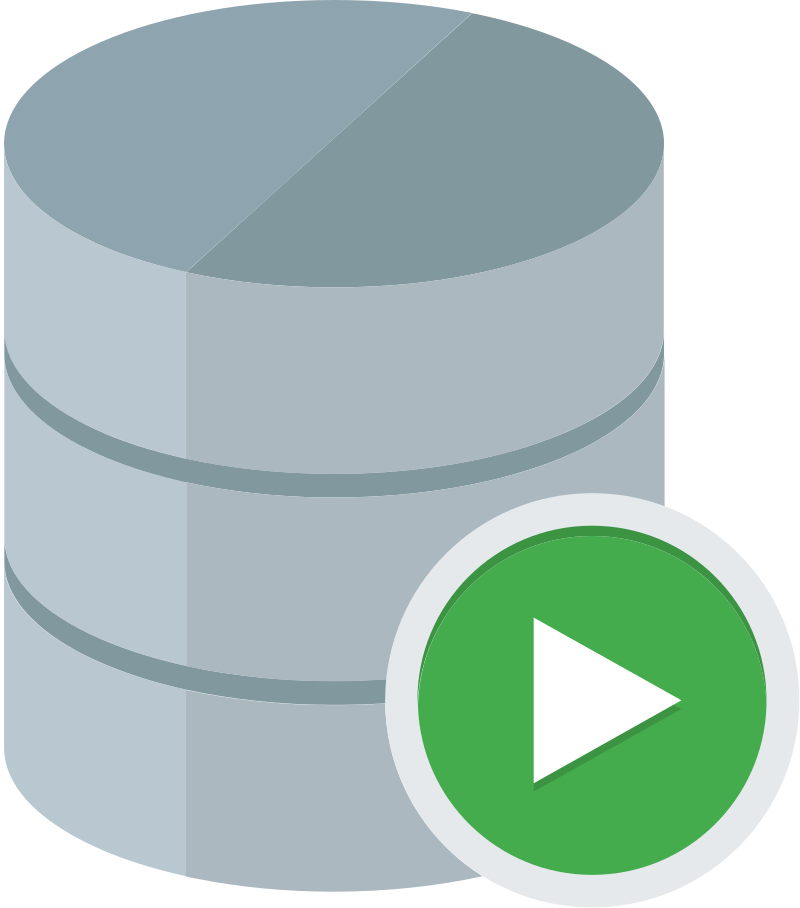
\includegraphics[width=0.18\textwidth]{logo-sqldeveloper}
    \caption{Logo SQL Developer}
    \label{fig:figure13}
    \end{center}
\end{figure}

%**************************************************************
\section{Organizzazione del testo}

\begin{description}
    \item[{\hyperref[cap:obbiettivi-pianificazione]{Il secondo capitolo}}] descrive gli obbietti dello stage, la pianificazione del lavoro effettuata a monte e le aspettative personali riguardanti lo stage;
    
    \item[{\hyperref[cap:metodologia-lavoro]{Il terzo capitolo}}] approfondisce la metodologia di lavoro e i ruoli adottati dal team di sviluppo;
    
    \item[{\hyperref[cap:prodotto-sw]{Il quarto capitolo}}] descrive dettagliatamente le funzionalità del software prodotto e le soluzioni adottate durante la codifica;
    
    \item[{\hyperref[cap:docs-test]{Il quinto capitolo}}] descrive la documentazione prodotta e i test eseguiti;
    
    \item[{\hyperref[cap:considerazioni]{Il sesto capitolo}}] contiene le considerazioni finali riguardanti lo stage e una valutazione personale sul lavoro svolto;

\end{description}

Riguardo la stesura del testo, relativamente al documento sono state adottate le seguenti convenzioni tipografiche:
\begin{itemize}
	\item gli acronimi, le abbreviazioni e i termini ambigui o di uso non comune menzionati vengono definiti nel glossario, situato alla fine del presente documento;
	\item per la prima occorrenza dei termini riportati nel glossario viene utilizzata la seguente nomenclatura: \emph{parola}\glsfirstoccur{};
	\item i termini in lingua straniera o facenti parti del gergo tecnico sono evidenziati con il carattere \emph{corsivo}.
\end{itemize}             % Introduzione
% !TEX encoding = UTF-8
% !TEX TS-program = pdflatex
% !TEX root = ../tesi.tex

%**************************************************************
\chapter{Obbiettivi e pianificazione}
\label{cap:obbiettivi-pianificazione}
%**************************************************************

\intro{In questo capitolo sono descritti gli obbiettivi dello stage, la pianificazione del lavoro e le aspettative personali.}\\

%**************************************************************
\section{Obbiettivi}
L'obbiettivo di questo stage è la realizzazione di una \textit{Proof of Concept} dell'applicazione, in cui vengono rese disponibili le funzionalità descritte in \hyperref[sez:scopo]{§1.2}. Per aumentare la produttività e permettere allo studente di conoscere nuove tecnologie viene utilizzato \textit{\hyperref[jhi]{JHipster}}. Lo studente verrà inserito in un gruppo di lavoro composto da 4 persone in modo da favorire, oltre alla comprensione delle nuove tecnologie, la capacità di lavorare in un \textit{team}.
Al termine del periodo di stage verrà effettuata una presentazione del prodotto alla direzione dell'azienda.
\\Nel piano di lavoro, documento la cui stesura è avvenuta prima dell'inizio dello stage, sono stati individuati i seguenti obbiettivi suddivisi in obbligatori, desiderabili e opzionali.
\subsection{Obbiettivi obbligatori}
\begin{itemize}
    \item Ob1: Conoscenza del \textit{framework Spring} e in particolare \textit{Spring MVC REST};
    \item Ob2: Interazione e gestione \textit{database Oracle};
    \item Ob3: Realizzazione delle funzionalità \textit{backend} del progetto.
\end{itemize}
\subsection{Obbiettivi desiderabili}
\begin{itemize}
    \item D1: Realizzazione delle funzionalità \textit{frontend} del progetto;
    \item D2: Conoscenza base sviluppo applicazioni \textit{frontend Angular};
    \item D3: Grado di autonomia nel processo di analisi/sviluppo.
\end{itemize}
\subsection{Obbiettivi opzionali}
\begin{itemize}
    \item Op1: Conoscenza base dei strumenti per \textit{\gls{ci}\glsfirstoccur{}/\gls{cd}\glsfirstoccur{}}.
\end{itemize}

%**************************************************************
\section{Pianificazione}
Lo stage prevede una durata di 312 ore complessive corrispondenti a 8 ore di lavoro giornalierio per un periodo di circa 8 settimane. L'orario di lavoro è dal Lunedì al Venerdì, dalle ore 9:00 alle 13:00 e dalle ore 14:00 alle 18:00. L'ora tra le 13:00 e le 14:00 è dedicata alla pausa pranzo.
\\La pianificazione redatta per il periodo di stage, divisa per obbiettivi settimanali, è la seguente:
\begin{itemize}
    \item \textbf{prima settimana:}
    \begin{itemize}
        \item studio strumenti di sviluppo (\textit{Eclipse, Maven, Git});
        \item analisi dei requisiti.
    \end{itemize}
    \item \textbf{seconda settimana:}
    \begin{itemize}
        \item creazione struttura del \textit{database};
        \item gestione \textit{database Oracle}.
    \end{itemize}
    \item \textbf{terza settimana:}
    \begin{itemize}
        \item studio e utilizzo del \textit{framework Spring};
        \item studio e utilizzo di \textit{Hibernate};
        \item realizzazione dell'\textit{object-relational mapping}. 
    \end{itemize}
    \item \textbf{quarta settimana:}
    \begin{itemize}
        \item utilizzo \textit{spring MVC} e \textit{Jackson};
        \item realizzazione dei servizi \textit{REST}.
    \end{itemize}
    \item \textbf{quinta settimana:}
    \begin{itemize}
        \item studio e utilizzo di elementi avanzati di \textit{Oracle};
        \item gestione \textit{changeset Liquibase};
        \item sviluppo di altri servizi \textit{REST}. 
    \end{itemize}
    \item \textbf{sesta settimana:}
    \begin{itemize}
        \item studio di \textit{Angular};
        \item sviluppo \textit{frontend};
    \end{itemize}
    \item \textbf{settima settimana:}
    \begin{itemize}
        \item \textit{\gls{ci}} e \textit{\gls{cd}};
        \item utilizzo di \textit{Sonarqube};
        \item controllo qualità del codice.
    \end{itemize}
    \item \textbf{ottava settimana:}
    \begin{itemize}
        \item gestione \textit{cache} dell'applicazione;
        \item ottimizzazione;
    \end{itemize}
\end{itemize}

%**************************************************************
\section{Aspettative personali}
Le mie aspettative per quanto riguarda lo stage erano molteplici.
\\Prima tra tutte la possibilità di lavorare in un'azienda che produce \textit{software} in modo da poter capire, almeno in parte, come funziona la vita in azienda.
In secondo luogo il mio obbiettivo era quello di imparare nuove tecnologie e le \textit{best practice} adottate dall'azienda ospitante, anche grazie alla stretta collaborazione con il mio \textit{tutor}.
Ultima cosa ma non meno importante è la possibilità di farsi conoscere da un azienda leader nel settore, in modo da poter pensare a eventuali collaborazioni future.             % Processi
% !TEX encoding = UTF-8
% !TEX TS-program = pdflatex
% !TEX root = ../tesi.tex

%**************************************************************
\chapter{Metodologia di sviluppo e composizione del team}
\label{cap:metodologia-lavoro}
%**************************************************************

\intro{Introduzione}\\

%**************************************************************
             % Kick-Off
%% !TEX encoding = UTF-8
% !TEX TS-program = pdflatex
% !TEX root = ../tesi.tex

%**************************************************************
\chapter{Analisi e progettazione}
\label{cap:analisi}
%**************************************************************

\intro{Il seguente capitolo descrive l'analisi, la progettazione iniziale, e le soluzioni addottate durante la codifica}\\


%**************************************************************
\section{Analisi e progettazione iniziale}
Le funzionalità da implementare e gli obbiettivi da raggiungere erano già ben definiti all'inizio del progetto, in quanto l'analisi funzionale è stata fornita dal Product owner insieme ad una prima definizione del product backlog.
Per questo motivo la fase di analisi dei requisiti da parte del team di sviluppo è stata molto breve e si è concentrata principalmente su come le funzionalità del prodotto dovessero essere fruibili all'utente finale. La progettazione del software non è avvenuta solamente all'inizio, ma si è protratta durante tutto il periodo di stage. Questo ha garantito maggior flessibilità nell'implementazione delle funzionalità e ha favorito l'utilizzo di Scrum. Tale scelta tuttavia ha anche introdotto il rischio che una debole progettazzione iniziale potesse causare problemi nelle settimane a venire. Questo rischio è stato subito mitigato grazie ad un attenta progettazione della base di dati pensando, nel miglior modo possibile, alle entità, a come esse fossero in relazione tra di loro e alla logica necessaria per implementare le funzionalità richieste. Inoltre, in quanto JHipster utilizza uno stack tecnologico ben definito, e impone dei vincoli architetturali da seguire, tale rischio è ulteriormente ridotto poiché non è necessario progettare l'architettura del prodotto.
Nel corso di questo capitolo vengono descritte le principali attività di progettazione svolte durante il corso dello stage.

%**************************************************************
\section{Progettazione del database}
La progettazione del database è stata una delle attività più importanti e deteneva un alto grado di priorità anche nel Product backlog. La progettazione del database è stata divisa in due parti: la prima mirata a individuare le entità partendo dall'analisi dei requisiti fatta dal Product owner, mentre la seconda mettendo in relazione tali entità aggiungendo tabelle se necessario. Per quanto riguarda la vera e propria implementazione del database è stato sfruttato un tool fornito da JHipster ovvero \href{https://start.jhipster.tech/jdl-studio/}{JDLStudio}, che verrà descritto in modo dettagliato successivamente nel corso di questa sezione.

\subsection{Entità}
Durante la progettazione della base di dati sono state definite le entità descritte di seguito.
Per ciascuna di esse viene riportata una breve descrizione e la lista dei suoi campi dati corredata da tipo di dato, nella lista seguente non vengono riportate chiavi primarie ne chiavi esterne poiché l'inserimento di tali campi dati è automatizzato e verrà descritto dettagliatamente nella sezione relativa alle \hyperref[rel]{relazioni tra entità}.
Mentre si stava effettuando la progettazione del database è sorto il problema di come si volessero salvare i \gls{contenutog} e i template. Si è optato di suddividere i contenuti in pagine, ognuna delle quali può contenere uno o più elementi multimediali e/o testuali. Inoltre in uno stesso contenuto si può selezionare un template diverso per ogni pagina. Per quanto riguarda i template, i quali sono definiti a monte dal team di sviluppo, si è scelto di strutturarli definendo un template al cui interno sono contenuti vari item che possono essere sia testuali che multimediali. Questo rende tutto il più modulare possibile, in quanto non pone limiti né in fase di creazione di un contenuto, né nella definizione dei template e nel loro utilizzo. 
\subsubsection{Content}
Definisce un contenuto informativo, i suoi campi dati sono:
\begin{itemize}
    \item name (String): Nome del contenuto;
    \item state (State): Enumerazione che definisce i possibili stati di un contenuto;
    \item description (String): descrizione del contenuto informativo;
    \item slideTime (Integer): durata delle slide di un contenuto;
\end{itemize}

\subsubsection{ContentPage}
Definisce una pagina inserita in un contenuto. Ogni contenuto può avere più pagine che scorreranno come slide durante la visualizzazione dello stesso; ogni pagina contiene degli item multimediali o testuali. I suoi campi dati sono:
\begin{itemize}
    \item pageNumber (Integer): numero della pagina all’interno di un contenuto.
\end{itemize}

\subsubsection{MultimediaItem}
Definisce un item multimediale (immagine o video) contenuto in una pagina. I suoi campi dati sono:
\begin{itemize}
    \item path (String): percorso del file multimediale caricato sul server, nel caso il caricamento delle immagini avvenga su NAS;
    \item resolution (Resolution): enumerazione che definisce la risoluzione dell'immagine caricata;
    \item multimediaFile (Blob): file multimediale caricato su database, nel caso il caricamento non avvenga su NAS;
\end{itemize}

\subsubsection{TextItem}
Definisce un testo contenuto in una pagina. I suoi campi dati sono:
\begin{itemize}
    \item text (Blob): contenuto testuale inserito in una pagina.
\end{itemize}

\subsubsection{Template}
Definisce un template che verrà utilizzato dalle pagine di un contenuto. Ogni pagina può utilizzare template definiti a monte che determinano come immagini, video e contenuti testuali vengono disposti nella pagina al momento della presentazione. I suoi campi dati sono:
\begin{itemize}
    \item previewImage (Blob): immagine di preview del template, utilizzata per aiutare l'utente a capire come questo è definito;
    \begin{figure}[h]
        \begin{center}
        
\includegraphics[width=0.18\textwidth]{textImage50_50}
        \caption{Immagine di preview di un template contenente un testo e un'immagine}
        \label{fig:figure15}
        \end{center}
    \end{figure}
    \item templateHTML (Blob): contiene l'html del template;
    \item name (String): Nome del template.
\end{itemize}

\subsubsection{TemplateItem}
Definisce un item all'interno di un template. Per item si intende un singolo testo, immagine o video. Questa entità viene utilizzata in fase di creazione e di visualizzazione di un contenuto ed è utilizzata per sapere cosa va inserito in una pagina che utilizza un determinato template. 
I suoi campi dati sono:
\begin{itemize}
    \item description (String): descrizione dell'item del template (e.g. video a schermo intero);
    \item type (itemType): enumerazione che definisce il contenuto che viene inserito in quell’area del template;
    \item TemplateArea (Integer): area del template in cui un certo oggetto va inserito, utilizzato in fase di preview per inserire immagini, video e testi al posto giusto all'interno del template.
\end{itemize}

\subsubsection{CSS}
Definisce il CSS utilizzato da uno o più template. I suoi campi dati sono:
\begin{itemize}
    \item templateCSS (Blob): contiene il CSS utilizzato da uno o più template.
\end{itemize}

\subsubsection{CustomAudit}
Entità definita per implementare il sistema di Audit. I suoi campi dati sono:
\begin{itemize}
    \item action (Action): enumerazione che definisce il tipo di azione registrata negli audit;
    \item description (String): descrizione dettagliata dell'azione effettuata;
    \item timestamp (Instant): data e ora in cui l'azione registrata è stata eseguita.
\end{itemize}

\subsubsection{User}
Entità predefinita in JHipster contenente tutte le informazioni necessarie per registrare un utente. Per utilizzarla è sufficiente definire relazioni ad essa.

\subsection{Enumerazioni}
Durante la progettazione della base di dati, in alcuni casi, si è ritenuto necessario definire alcuni campi dati come enumerazione al posto di utilizzare una semplice stringa di testo.
Questo garantisce maggior controllo e impone vincoli che evitano il verificarsi di errori relativi all'utilizzo di nomi diversi per esprimere lo stesso concetto. Le enumerazioni definite durante la progettazione del database sono le seguenti.

\subsubsection{State}
Lista dei possibili stati di un contenuto informativo, ovvero: \textit{CREATED, TO\textunderscore{}ASSOCIATE, ASSOCIATED, TO\textunderscore{}AUTHORIZE, AUTHORIZED, PUBLISHED}.

\subsubsection{Resolution}
Lista delle possibili risoluzioni di un elemento multimediale, ovvero: \textit{HIGH, MEDIUM, LOW}.

\subsubsection{ItemType}
Lista delle diverse tipologie di template item, ovvero: \textit{IMAGE, VIDEO, TEXT}.

\subsubsection{Action}
Lista delle azioni da registrare nel sistema di auditing che possono essere effettuate da un utente, ovvero: \textit{CREATE, DELETE, UPDATE, AUTHENTICATION\textunderscore{}SUCCESS, AUTHENTICATION\textunderscore{}FAILURE, LOGOUT, TIMEOUT}.

\subsection{Relazioni}
\label{rel}
Di seguito vengono evidenziate le relazioni tra le entità descritte in precedenza e ne viene data una breve descrizione.
\subsubsection{Content-ContentPage}
Ogni Content può avere una o più ContentPage, ogni ContentPage è inserita in un solo contenuto.
\subsubsection{Template-ContentPage}
Ogni Template può essere utilizzato da una o più ContentPage, ogni ContentPage utilizza un solo Template.
\subsubsection{Content-page-MultimediaItem}
Ogni ContentPage può contenere uno o più MultimediaItem, ogni MultimediaItem è contenuto in una sola pagina.
\subsubsection{ContentPage-TextItem}
Ogni ContentPage può contenere uno o più TextItem, ogni TextItem è contenuto in una sola pagina.
\subsubsection{Template-TemplateItem}
Ogni Template ha al suo interno uno o più TemplateItem, ogni TemplateItem fa riferimento a un solo Template.
\subsubsection{MultimediaItem-TemplateItem}
Ogni MultimediaItem può riferirsi ad un solo TemplateItem, ad ogni TemplateItem possono essere riferiti uno o più MultimediaItem.
\subsubsection{TextItem-TemplateItem}
Ogni TextItem può riferirsi ad un solo TemplateItem, ad ogni TemplateItem possono essere riferiti uno o più TextItem.
\subsubsection{Content-User}
Ogni Content è creato da un solo User, ogni User può creare uno o più content.
\subsubsection{CSS-Template}
Ogni Template può avere uno o più CSS, ogni CSS può essere utilizzato da uno o più Template.
\subsubsection{CustomAudit-User}
Ogni Audit si riferisce ad un solo User, ad ogni User possono essere registrati uno o più Audit.


\subsection{Implementazione}
\subsubsection{JDL Studio}
JDL Studio è un tool fornito da JHipster che permette di definire lo schema entità-relazioni di un database tramite un apposito linguaggio di scripting chiamato, appunto, JDL. Una delle funzionalità più utili di JDLStudio è la possibilità di visualizzare il modello ER, che viene automaticamente aggiornato ad ogni modifica.
\newpage
\subsubsection{Definizione di un'entità in JDLStudio}
Un'entità viene definita in JDL specificando il suo nome e i suoi campi dati. Un esempio di definizione di un'entità è il seguente:
\begin{lstlisting}[caption={Definizione entità Content},label={lst:ent}]
entity Content {
  name String unique,
  state State,
  description String,
  slideTime Integer
}
\end{lstlisting}
\subsubsection{Definizione di un'enumerazione in JDLStudio}
Un'enumerazione viene definita in JDL specificandone il nome e i suoi possibili valori dati. Un esempio di definizione di un'entità è il seguente:
\begin{lstlisting}[caption={Definizione enumerazione State},label={lst:ent}]
enum State {
  CREATED,
  TO_ASSOCIATE,
  ASSOCIATED,
  TO_AUTHORIZE,
  AUTHORIZED,
  PUBLISHED
}
\end{lstlisting}
\subsubsection{Definizione di una relazione in JDLStudio}
Per definire una relazione in JDL bisogna innanzitutto specificare il tipo di relazione (uno a uno, uno a molti, molti a molti). Fatto questo è sufficiente specificare l'entità di partenza della relazione e quella di arrivo. Un esempio di definizione di relazioni in JDL è il seguente:
\begin{lstlisting}[caption={Definizione relazioni uno a molti},label={lst:ent}]
relationship OneToMany {
  Content{page} to ContentPage{content},
  Template{page} to ContentPage{template},
  ContentPage{multimediaItem} to MultimediaItem{page},
  TemplateItem{multimediaItem} to MultimediaItem{templateItem},
  Template{templateItem} to TemplateItem{template},
  ContentPage{textItem} to TextItem{page},
  TemplateItem{textItem} to TextItem{templateItem}
}
\end{lstlisting}
\newpage
\subsubsection{Modello ER}
Il modello ER autogenerato presenta imperfezioni nella visualizzazione delle relazioni, nonostante ciò e stato ritenuto sufficiente per gli scopi del progetto.
\begin{figure}[h]
    \begin{center}
    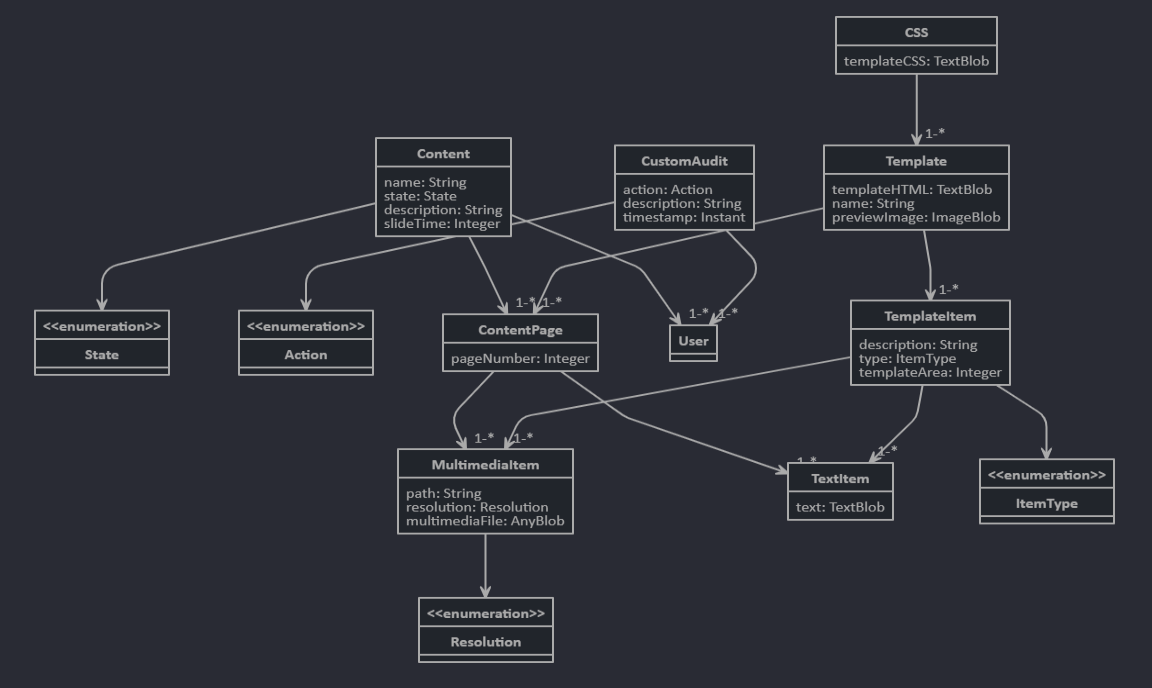
\includegraphics[width=1.2\textwidth]{er}
    \caption{Modello ER generato da JDLStudio}
    \label{fig:figure19}
    \end{center}
\end{figure}

%**************************************************************
\section{Definizione dei template per i contenuti}
In quanto nella progettazione del database è stato scelto di modellare i template in modo che fossero più modulari ed estendibili possibile, è stata necessaria un accurata definizione degli stessi. Si è optato per definire un template di base utilizzato da ogni contenuto informativo, e una serie di template personalizzati utilizzati dalle pagine inserite in un contenuto.
\subsection{Template di base}
Il template di base definito contiene poche informazioni. Definisce infatti la struttura base della pagina html e la funzione per visualizzare le slide. Contiene inoltre vari placeholder utilizzati per inserire dinamicamente le informazioni di un determinato contenuto informativo.
I placeholder definiti sono: 

%**************************************************************
\section{Definizione dei servizi di backend}

             % Concept Preview
%% !TEX encoding = UTF-8
% !TEX TS-program = pdflatex
% !TEX root = ../tesi.tex

%**************************************************************
\chapter{Prodotto}
\label{cap:prodotto}
%**************************************************************

\intro{In questo capitolo viene descritto il prodotto software, la documentazione e i test eseguiti.}\\

%**************************************************************
\section{Prodotto software}
Nel corso di questa sezione vengono descritte tutte le funzionalità implementate al momento del termine dello stage.

\subsection{Login}
Il \textit{login} del prodotto finale dovrà essere gestito tramite un sistema di \gls{ssog} esterno. Nonostante ciò l'implementazione di tale sistema non era tra gli obbiettivi di stage, per la demo finale è stato ritenuto sufficiente utilizzare un \gls{mockg} dello stesso. 
\begin{figure}[h]
    \begin{center}
    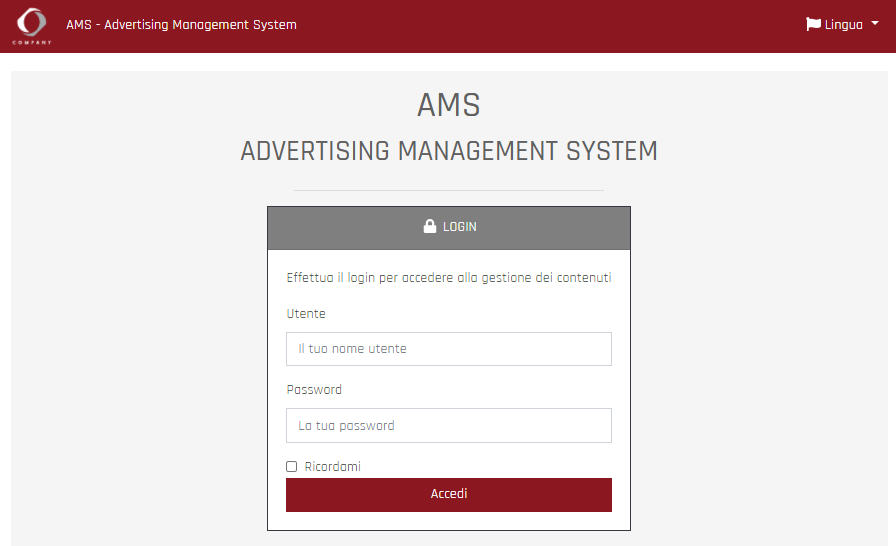
\includegraphics[width=0.95\textwidth]{login}
    \caption{Schermata di login}
    \label{fig:figure20}
    \end{center}
\end{figure}

\subsection{Scelta funzionalità}
La schermata principale del prodotto è la schermata di scelta funzionalità. Tramite questa schermata si possono raggiungere le varie funzioni offerte dal prodotto.
\begin{figure}[h]
    \begin{center}
    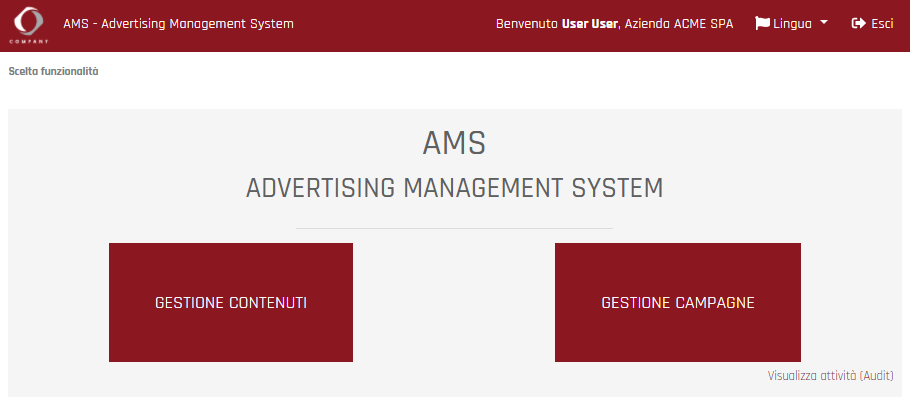
\includegraphics[width=1\textwidth]{funzionalita}
    \caption{Schermata di scelta funzionalità}
    \label{fig:figure21}
    \end{center}
\end{figure}
Più nello specifico, le funzionalità raggiungibili tramite questa schermata sono:
\begin{itemize}
    \item gestione dei contenuti;
    \item gestione delle campagne (Non abilitata);
    \item visualizzazione \textit{audit}.
\end{itemize}

\subsection{Gestione contenuti}
Tramite la schermata di gestione contenuti è possibile raggiungere le sezioni di lavoro divise per ruolo (Editore, Redattore, Supervisore).
\begin{figure}[h]
    \begin{center}
    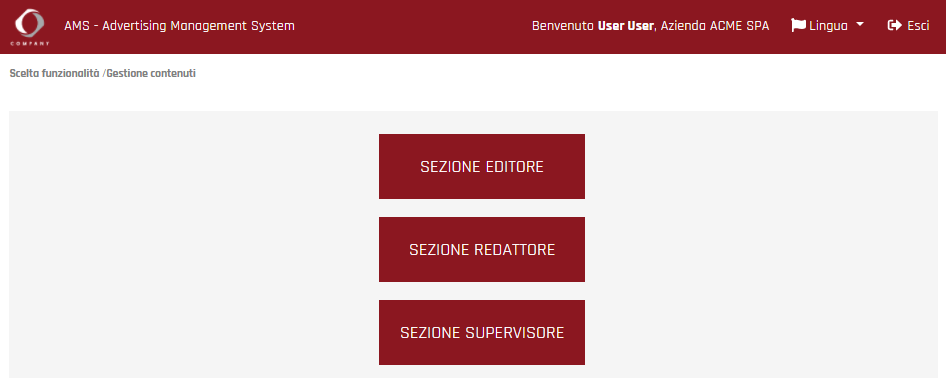
\includegraphics[width=1\textwidth]{gestcont}
    \caption{Schermata di gestione contenuti}
    \label{fig:figure22}
    \end{center}
\end{figure}
\\Ovviamente ogni utente puo visualizzare solamente le sezioni relative ai ruoli a lui assegnati.

\subsection{Sezione editore}
Questa sezione è quella in cui sono utilizzabili la maggior parte delle funzionalità obbiettivo dello stage. In questa schermata è visualizzata una lista di tutti i \gls{contenutog}. Per ciascuno di questi è possibile:
\begin{itemize}
    \item visualizzarne l'anteprima;
    \item clonarlo;
    \item modificarlo;
    \item richiederne l'associazione;
    \item eliminarlo.
\end{itemize}
Nel caso sia stata richiesta l'associazione di un contenuto, questo non potra più essere eliminato né modificato.
Tramite questa pagina è inoltre possibile creare un nuovo contenuto.
\begin{figure}[h]
    \begin{center}
    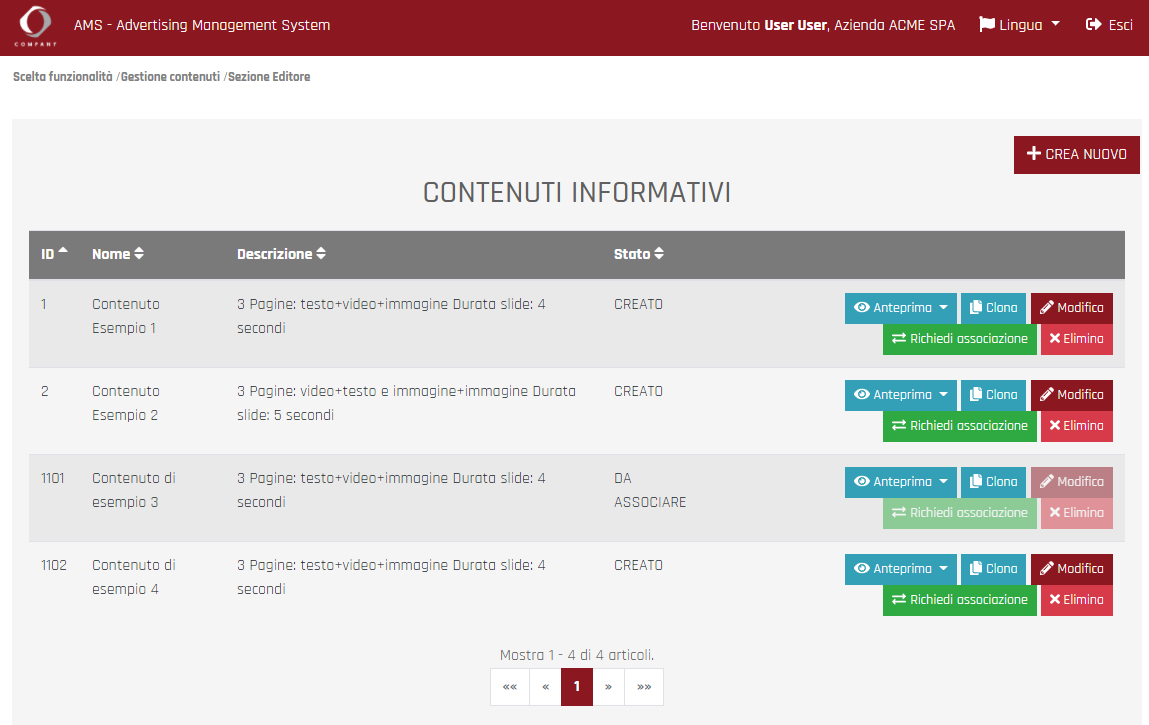
\includegraphics[width=1\textwidth]{editore}
    \caption{Schermata di gestione contenuti}
    \label{fig:figure23}
    \end{center}
\end{figure}

\subsection{Creazione di un contenuto}
La schermate di creazione di un contenuto è divisa in due aree. In quella di sinistra si inseriscono le informazioni generali relative al contenuto. In quella di destra è possibile creare le pagine del contenuto, selezionando per ciascuna uno tra i vari \textit{template} disponibili.
Nel caso si scelgano \textit{template} con contenuti multimediali è sufficiente che questi vengano caricati attraverso l'apposito pulsante. Nel caso ci siano contenuti testuali da inserire è possibile invece utilizzare l'apposito editor di testo.
\begin{figure}[h]
    \begin{center}
    \includegraphics[width=1\textwidth]{Creazione}
    \caption{Creazione di un contenuto}
    \label{fig:figure24}
    \end{center}
\end{figure}

\subsection{Anteprima di un contenuto}
La possibilità di visualizzare l'anteprima di un contenuto una volta creato è una delle funzionalità più utili e importanti. L'anteprima permette infatti di visualizzare come si presenterebbe un contenuto una volta pubblicato e permette di decidere se richiederne l'associazione o modificarlo.
\begin{figure}[h]
    \begin{center}
    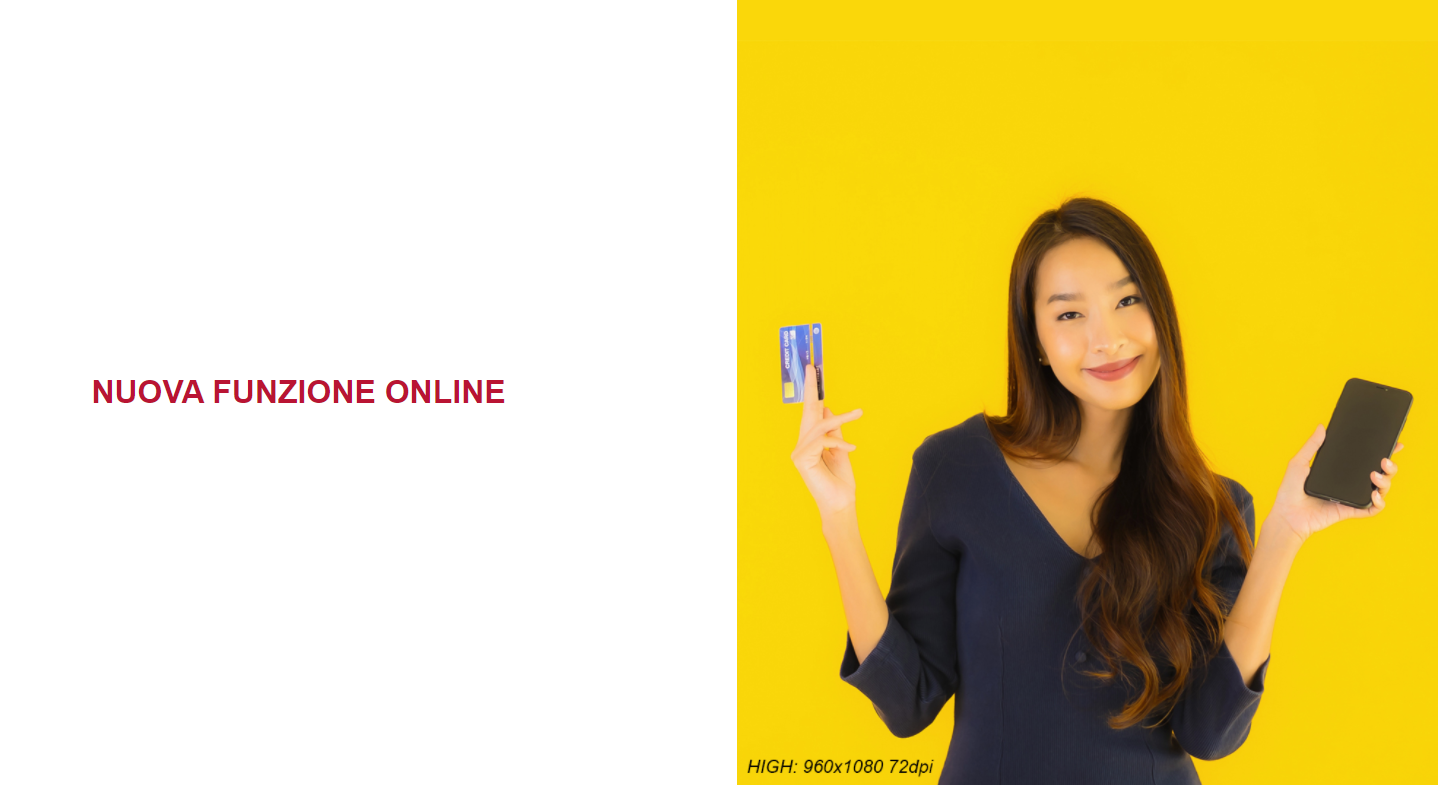
\includegraphics[width=1\textwidth]{anteprima}
    \caption{Anteprima di un contenuto di esempio}
    \label{fig:figure25}
    \end{center}
\end{figure}

\subsection{Clonazione di un contenuto}
La possibilità di clonare un contenuto è utile nel caso si voglia creare un contenuto simile ad uno già pubblicato senza la necessità di dover partire da zero. Per clonare un contenuto è sufficiente cliccare su \textit{"Clona"} nella sezione dedicata al ruolo di editore. Fatto ciò si aprirà automaticamente un pannello modale in cui è necessario inserire il nome che si vuole assegnare al nuovo contenuto.
\begin{figure}[h]
    \begin{center}
    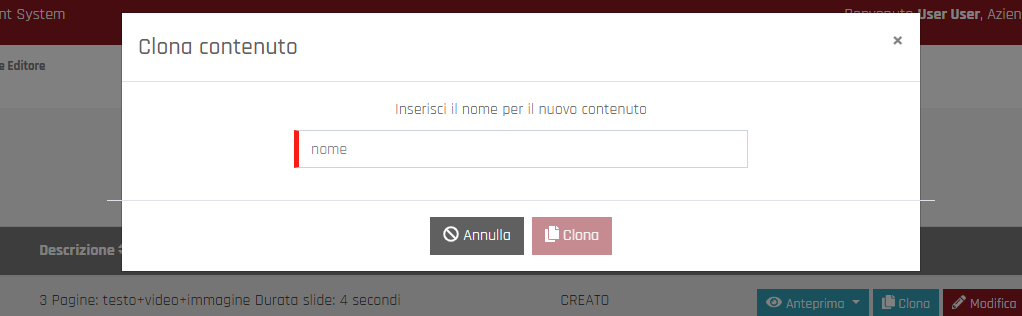
\includegraphics[width=1\textwidth]{clona}
    \caption{Clonazione di un contenuto}
    \label{fig:figure26}
    \end{center}
\end{figure}

\subsection{Modifica di un contenuto}
Modificare un contenuto può essere indispensabile nel caso, ad esempio, siano state inserite immagini o testi errati. La schermata di modifica di un contenuto si presenta in modo analogo a quella di creazione con la differenza che i campi dati hanno già le informazioni del contenuto al loro interno.
\begin{figure}[h]
    \begin{center}
    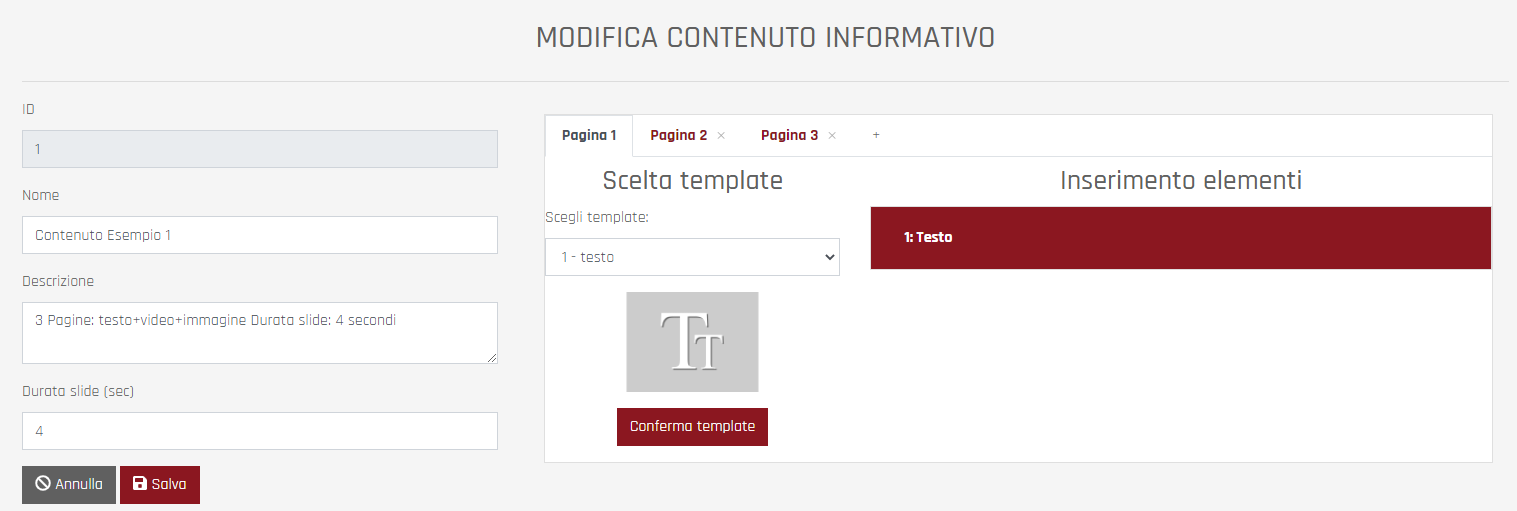
\includegraphics[width=1\textwidth]{modifica}
    \caption{Modifica di un contenuto}
    \label{fig:figure27}
    \end{center}
\end{figure}
\newpage
\subsection{Associazione di un contenuto}
La richiesta di associazione di un contenuto è il primo passo da eseguire perchè questo possa essere pubblicato. Una volta richiesta l'associazione di un contenuto questo non potrà più essere modificato ne eliminato. L'associazione può essere approvata o rifiutata da un redattore; nel primo caso il contenuto potrà proseguire nel suo ciclo di vita, nel secondo tornerà allo stato iniziale e sarà di nuovo modificabile.
\begin{figure}[h]
    \begin{center}
    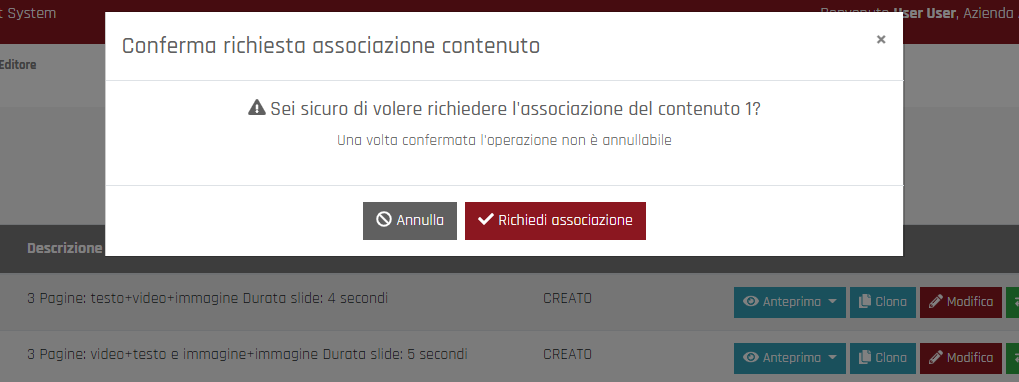
\includegraphics[width=1\textwidth]{associazione}
    \caption{Richiesta di associazione di un contenuto}
    \label{fig:figure28}
    \end{center}
\end{figure}

\subsection{Eliminazione di un contenuto}
Un contenuto potrebbe essere creato per errore o non più necessario, in questo caso può tornare utile l'eliminazione. L'eliminazione è irreversibile.
\begin{figure}[h]
    \begin{center}
    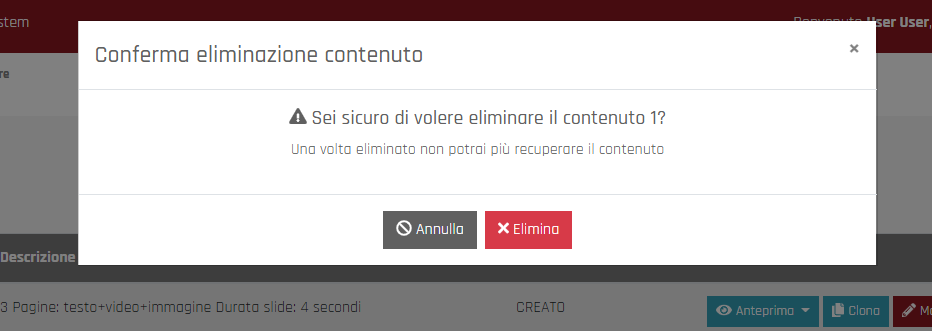
\includegraphics[width=1\textwidth]{eliminazione}
    \caption{Eliminazione di un contenuto}
    \label{fig:figure29}
    \end{center}
\end{figure}

\subsection{Audit}
La schermata di visualizzazione degli \textit{audit}, raggiungibile dalla schermata principale, è visualizzabile da chiunque abbia effetuato il \textit{Login} e raccoglie varie informazioni sulle attività effettuate dagli utenti.
\begin{figure}[h]
    \begin{center}
    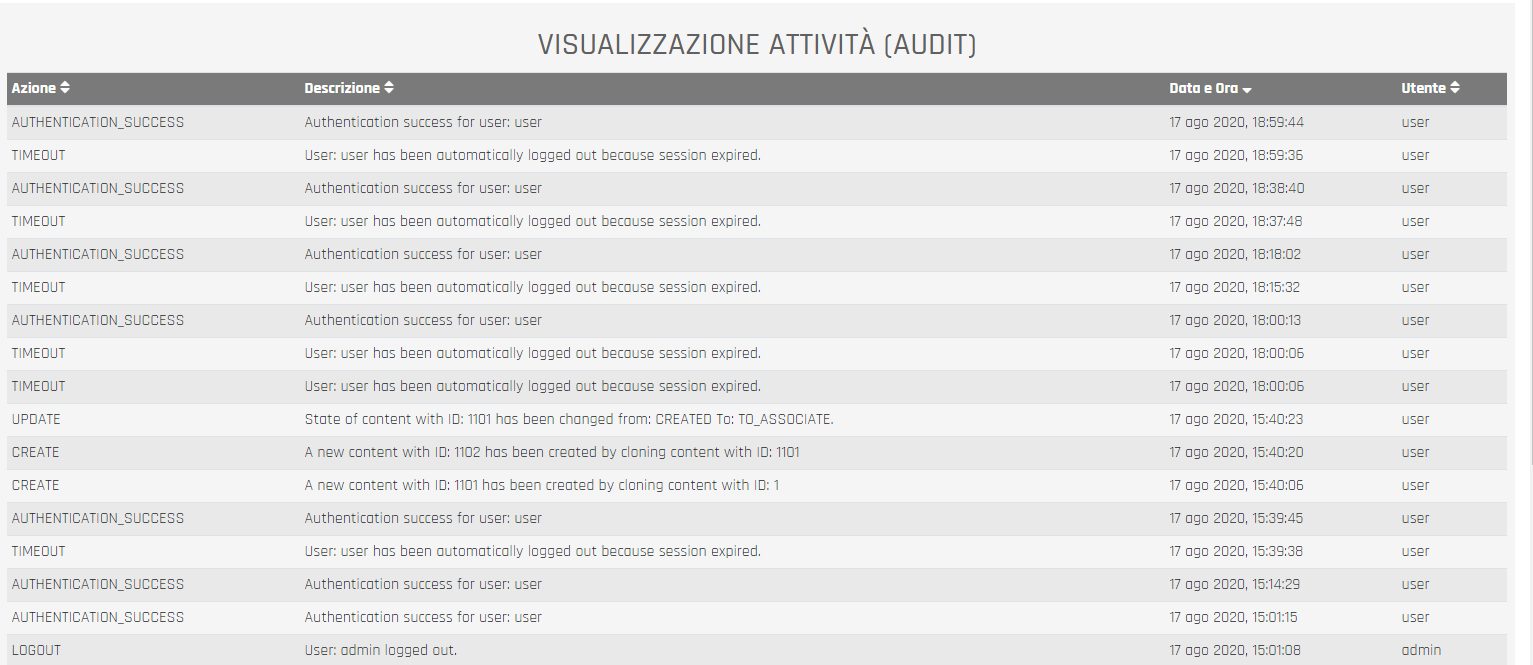
\includegraphics[width=1\textwidth]{audit}
    \caption{Visualizzazione audit}
    \label{fig:figure30}
    \end{center}
\end{figure}

%**************************************************************
\section{Documentazione}
Oltre allo sviluppo dell'applicazione vera e propria una parte delle ore a disposizione è stata dedicata alla documentazione. In accordo con il \textit{Product Owner} è stato deciso di redarre solamente il manuale utente e il manuale sviluppatore.

\subsection{Manuale Utente}
Lo scopo di questo documento è illustrare tutte le funzionalità del prodotto. In tal modo l'utente finale ha a disposizione tutte le informazione per utilizzare il \textit{software} correttamente.
Il manuale utente descrive:
\begin{itemize}
    \item requisiti di sistema;
    \item utilizzo dell'applicazione.
\end{itemize}

\subsection{Manuale Sviluppatore}
Lo scopo di questo documento è illustrare le scelte implementative effettuate durante lo sviluppo e dare informazioni utili ad uno sviluppatore che comincia a lavorare a questo progetto.
Il manuale sviluppatore tuttavia non ha lo scopo di sostituirsi alla documentazione ufficiale delle tecnologie utilizzate. Per tale motivo all'interno di esso sono contenuti numerosi riferimenti a documenti esterni.
Il manuale sviluppatore descrive:
\begin{itemize}
    \item setup dell'ambiente di lavoro;
    \item gestione delle dipendenze \textit{Angular};
    \item gestione della dipendenza ad \textit{Oracle};
    \item utilizzo di \textit{Angular CLI};
    \item \textit{build} e \textit{packaging} dell'applicazione;
    \item \textit{testing};
    \item utilizzo di \textit{Docker};
    \item \gls{ci};
    \item scelte implementative effettuate.
\end{itemize}

%**************************************************************
\section{Test}
Nello sviluppo di un'applicazione il \textit{testing} è una delle fasi più importanti. Poiché ogni due settimane veniva presentata una demo dell'applicativo i \textit{test} sono stati eseguiti di continuo durante lo sviluppo, sia in modo automatico che non. Nel corso di questa sezione vengono descritti i \textit{test} svolti durante lo sviluppo.

\subsection{Test di unità}
I \textit{test} di unità sono eseguiti per verificare se sono presenti errori nei singoli metodi. Nel corso dello stage i \textit{test} di unità sono stati eseguiti tramite \textit{JUnit} e \textit{Jest}. Tali \textit{framework} sono sviluppati rispettivamente per \textit{Java} e per \textit{Javascript}. Il primo è stato utilizzato per testare il \textit{back-end} mentre il secondo per il \textit{front-end}.

\begin{lstlisting}[caption={Test di unità in Java},label={utj}]
    @Test
    @Transactional
    public void createContent() throws Exception {
        int databaseSizeBeforeCreate = contentRepository.findAll().size();
        // Create the Content
        restContentMockMvc.perform(post("/api/contents")
            .contentType(MediaType.APPLICATION_JSON)
            .content(TestUtil.convertObjectToJsonBytes(content)))
            .andExpect(status().isCreated());

        // Validate the Content in the database
        List<Content> contentList = contentRepository.findAll();
        assertThat(contentList).hasSize(databaseSizeBeforeCreate + 1);
        Content testContent = contentList.get(contentList.size() - 1);
        assertThat(testContent.getName()).isEqualTo(DEFAULT_NAME);
        assertThat(testContent.getState()).isEqualTo(DEFAULT_STATE);
        assertThat(testContent.getDescription()).isEqualTo(DEFAULT_DESCRIPTION);
        assertThat(testContent.getSlideTime()).isEqualTo(DEFAULT_SLIDE_TIME);
    }
\end{lstlisting}
\newpage
\begin{lstlisting}[caption={Test di unità in JavaScript},label={utj}]
    describe('Component Tests', () => {
  describe('Home Component', () => {
    let comp: HomeComponent;
    let fixture: ComponentFixture<HomeComponent>;
    let accountService: AccountService;
    let loginModalService: LoginModalService;

    beforeEach(async(() => {
      TestBed.configureTestingModule({
        imports: [AmsTestModule],
        declarations: [HomeComponent],
      })
        .overrideTemplate(HomeComponent, '')
        .compileComponents();
    }));

    beforeEach(() => {
      fixture = TestBed.createComponent(HomeComponent);
      comp = fixture.componentInstance;
      accountService = TestBed.get(AccountService);
      loginModalService = TestBed.get(LoginModalService);
    });

    it('Should call accountService.getAuthenticationState on init', () => {
      // WHEN
      comp.ngOnInit();

      // THEN
      expect(accountService.getAuthenticationState).toHaveBeenCalled();
    });

    it('Should call accountService.isAuthenticated when it checks authentication', () => {
      // WHEN
      comp.isAuthenticated();

      // THEN
      expect(accountService.isAuthenticated).toHaveBeenCalled();
    });

    it('Should call loginModalService.open on login', () => {
      // WHEN
      comp.login();

      // THEN
      expect(loginModalService.open).toHaveBeenCalled();
    });
  });
});
\end{lstlisting}

\subsection{Test di integrazione}
I \textit{test} di integrazione vengono eseguiti per verificare che non ci siano errori di integrazione tra le varie componenti del sistema. Nel corso del progetto questa fase di \textit{test} è stata ritenuta di grande importanza, in particolare nell'integrazione tra il \textit{back-end} e il \textit{front-end}. In questo caso i suddetti \textit{test} sono stati eseguiti manualmente. 

\subsection{Test di sistema}
I \textit{test} di sistema vengono eseguiti per assicurare che il sistema soddisfi i requisiti richiesti. Nel corso dello stage dopo l'implementazione di una nuova funzionalità l'intero sistema veniva testato. Al termine di ogni sprint tali \textit{test} venivano eseguiti dal \textit{product owner}, in tal caso questi possono essere considerati \textit{test} di accettazione.

\subsection{Test di performance}
I \textit{test} di performance vengono eseguiti per controllare che il sistema non risulti lento durante il suo utilizzo. Tali \textit{test} sono stati eseguiti con l'ausilio del pannello amministratore generato da \textit{JHipster}. Questo permette di visualizzare una moltitudine di informazioni come ad esempio le risorse occupate o il tempo di esecuzione delle \gls{apig}.
\begin{figure}[h]
    \begin{center}
    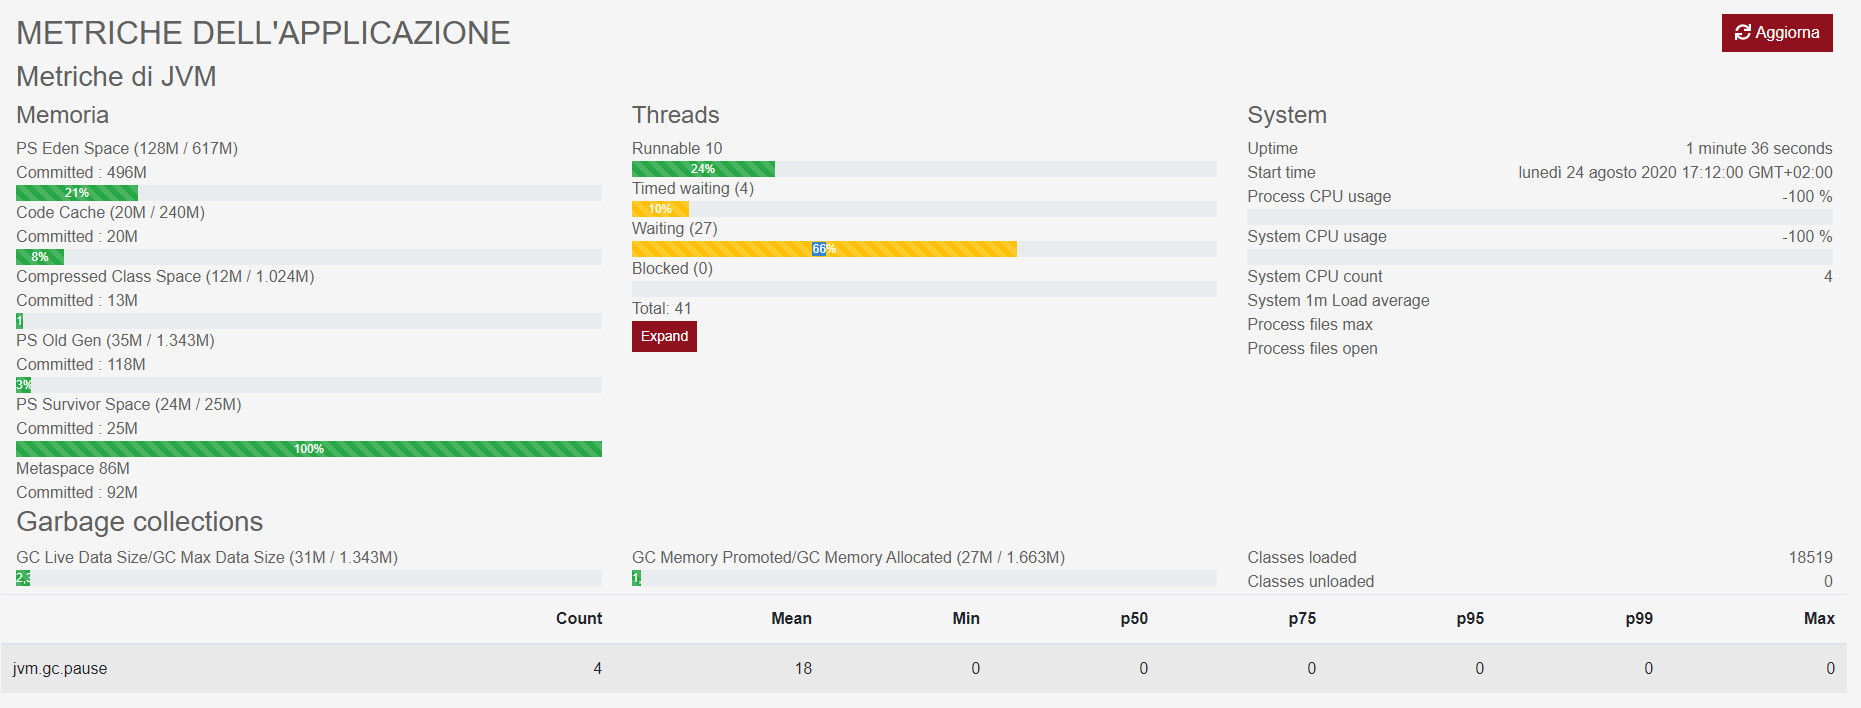
\includegraphics[width=1\textwidth]{metriche1}
    \caption{Metriche dell'applicazione}
    \label{fig:figure31}
    \end{center}
\end{figure}

\section{Accessibilità}
I \textit{test} di accessibilità sono necessari per verificare che l'applicativo risulti utilizzabile anche da utenti con disabilità. Nel corso del progetto si è cercato di attenersi alle regole definite nello standard \href{https://www.w3.org/TR/WCAG21/}{WCAG 2.1}. I test veri e propri sono stati poi eseguiti tramite \href{https://developers.google.com/web/tools/lighthouse/?utm_source=devtools}{\textit{Lighthouse}}, un tool per l'analisi dinamica di pagine web.             % Product Prototype
%% !TEX encoding = UTF-8
% !TEX TS-program = pdflatex
% !TEX root = ../tesi.tex

%**************************************************************
\chapter{Considerazioni finali}
\label{cap:considerazioni}
%**************************************************************

\intro{Introduzione}\\

%**************************************************************
             % Product Design Freeze e SOP
%\input{capitoli/capitolo-7}             % Conclusioni
\appendix                               
%\input{capitoli/capitolo-A}             % Appendice A

%**************************************************************
% Materiale finale
%**************************************************************
\backmatter
\printglossaries
% !TEX encoding = UTF-8
% !TEX TS-program = pdflatex
% !TEX root = ../tesi.tex

%**************************************************************
% Bibliografia
%**************************************************************

\cleardoublepage
\chapter{Bibliografia}

\nocite{*}
% Stampa i riferimenti bibliografici
\printbibliography[heading=subbibliography,title={Riferimenti bibliografici},type=book]

% Stampa i siti web consultati
\printbibliography[heading=subbibliography,title={Siti web consultati},type=online]


\end{document}
